\documentclass[green, compress]{beamer}
\usepackage[spanish, activeacute]{babel}
\usepackage[utf8]{inputenc}
\usepackage{beamerthemesplit}
\usepackage{beamerthemeshadow}
\usepackage{multirow}
\usepackage{array}
\usepackage{colores}

\usetheme{Darmstadt}

\beamertemplateshadingbackground{orange!30}{white!80}

\useinnertheme{rounded}
\setbeamercovered{transparent}

\usecolortheme[named=verde]{structure}

\AtBeginSubsection[]
{
  \begin{frame}<beamer>
    \frametitle{Índice}
    \tableofcontents[currentsection,currentsubsection]
  \end{frame}

}

\title{FreePhyloTree}
\author[A. Bueno]{Aarón Bueno Villares \\ \textit{\tiny abv150ci@gmail.com}}
\date{}

\begin{document}

\begin{frame}
  \titlepage

\begin{center}
  \begin{tabular}{m{3cm} @{\hspace{1cm}} m{3cm}}
    \makebox[2.5cm][c]{
\includegraphics[scale=.1]{logo_uca.png}} &
    \makebox[2.5cm][c]{
\includegraphics[scale=.5]{cc-by-sa.png}}
  \end{tabular}
\end{center}

\end{frame}

\section{Introducción}
\begin{frame}
\frametitle{FreePhyloTree}
\begin{center}
  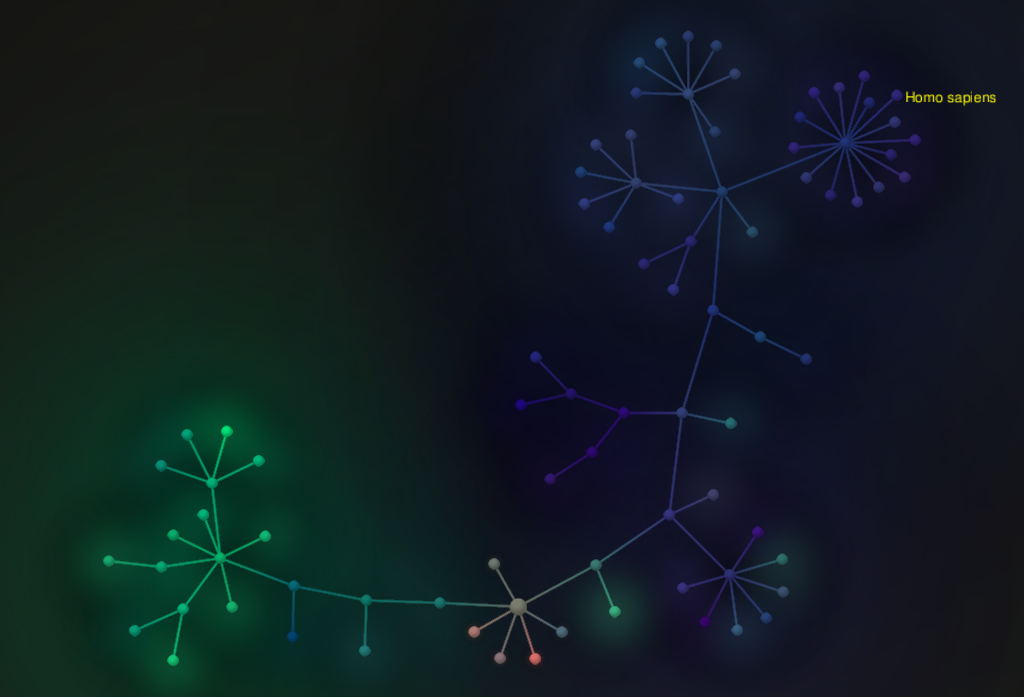
\includegraphics[scale=.3]{capture.png}
\end{center}
\end{frame}

\section{Conceptos}

\begin{frame}
\frametitle{Árbol filogenético}
\begin{center}
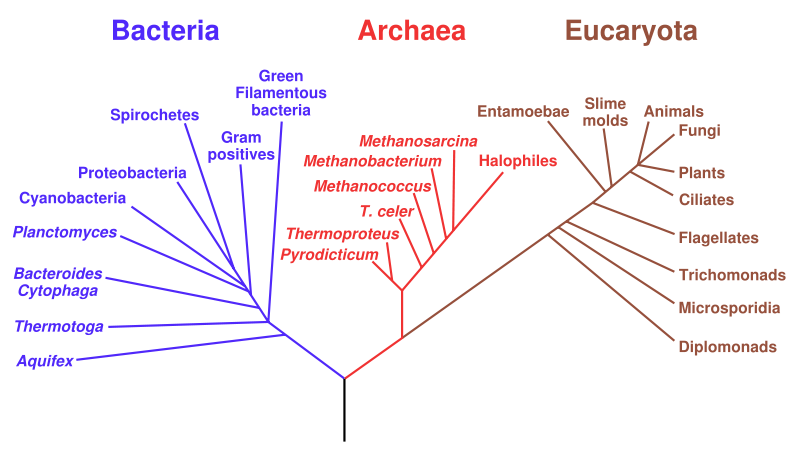
\includegraphics[scale=.3]{phylogeneticTree.png}
\end{center}
\end{frame}

\begin{frame}
\frametitle{Cladograma}
\begin{center}
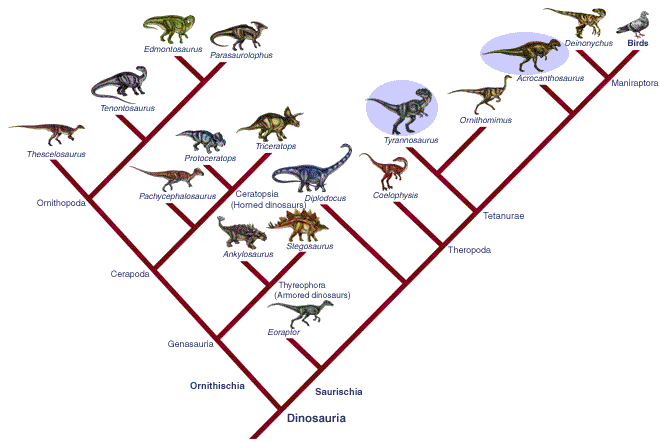
\includegraphics[scale=.4]{cladogramDino.png}
\end{center}
\end{frame}

\begin{frame}
\frametitle{Clasificación}
\begin{block}{Taxonomía}
\begin{itemize}
\item Reglas de clasificación.
\item Nivel jerárquico: (Dominio) - Reino - Filo - Clase - Órden -
  Familia - Género - Especie.
\end{itemize}
\end{block}

\begin{block}{Sistemática}
\begin{description}
\item[Fenética:] Clasificación según rasgos morfológico.
\item[Cladística:] Clasificación basada en árboles filogenéticos.
\item[Sistemática evolutiva:] Clasificación basada en árboles
  filogenéticos con «modificaciones».
\end{description}
\end{block}
\end{frame}

\section{Softwares existentes}

\begin{frame}{Archaeopteryx - LGPL}
\begin{center}
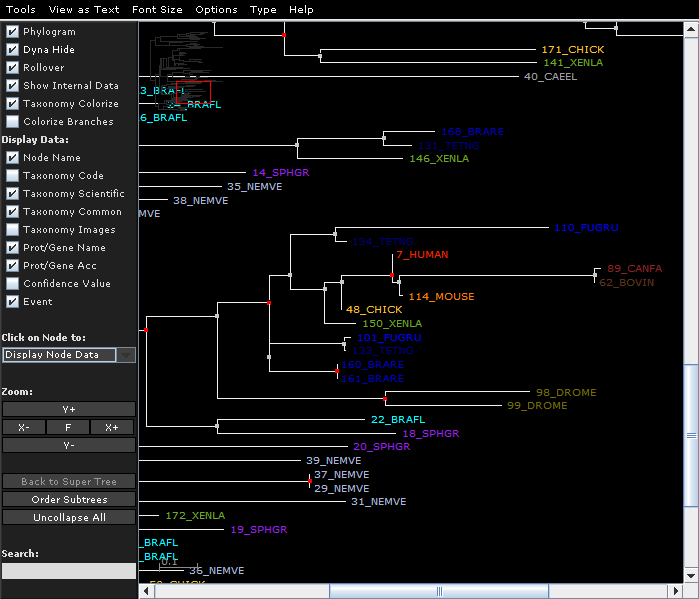
\includegraphics[scale=.3]{bcl2.png}
\end{center}
\end{frame}

\begin{frame}{Dendroscope (uso bajo licencia)}
\begin{center}
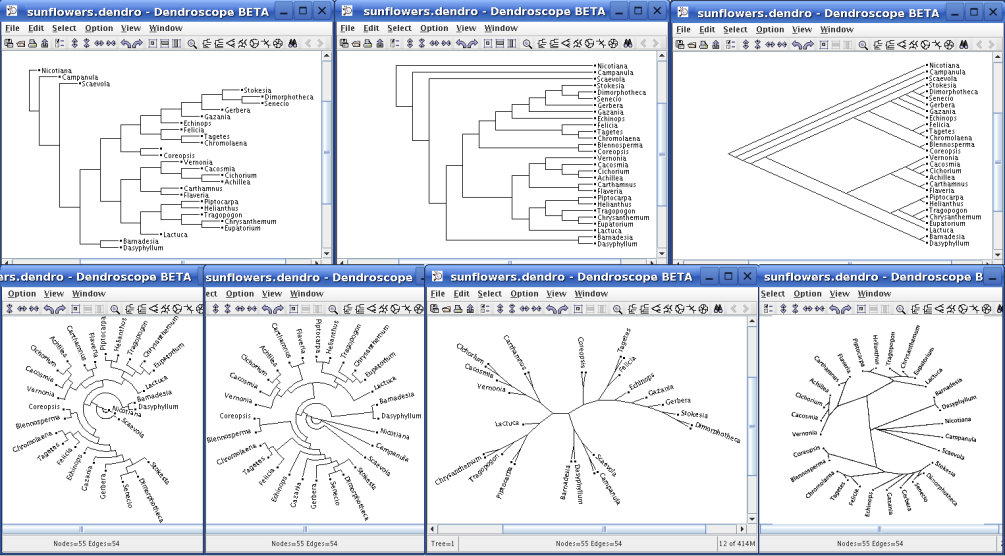
\includegraphics[scale=.3]{7views.png}
\end{center}
\end{frame}

\begin{frame}{A Python Enviroment for Tree Exploration (E.T.E) - GPL}
\begin{center}
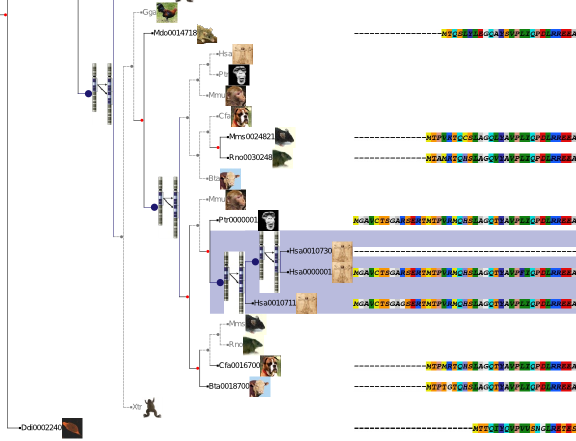
\includegraphics[scale=.5]{ETE.png}
\end{center}
\end{frame}

\begin{frame}{Figtree}
\begin{center}
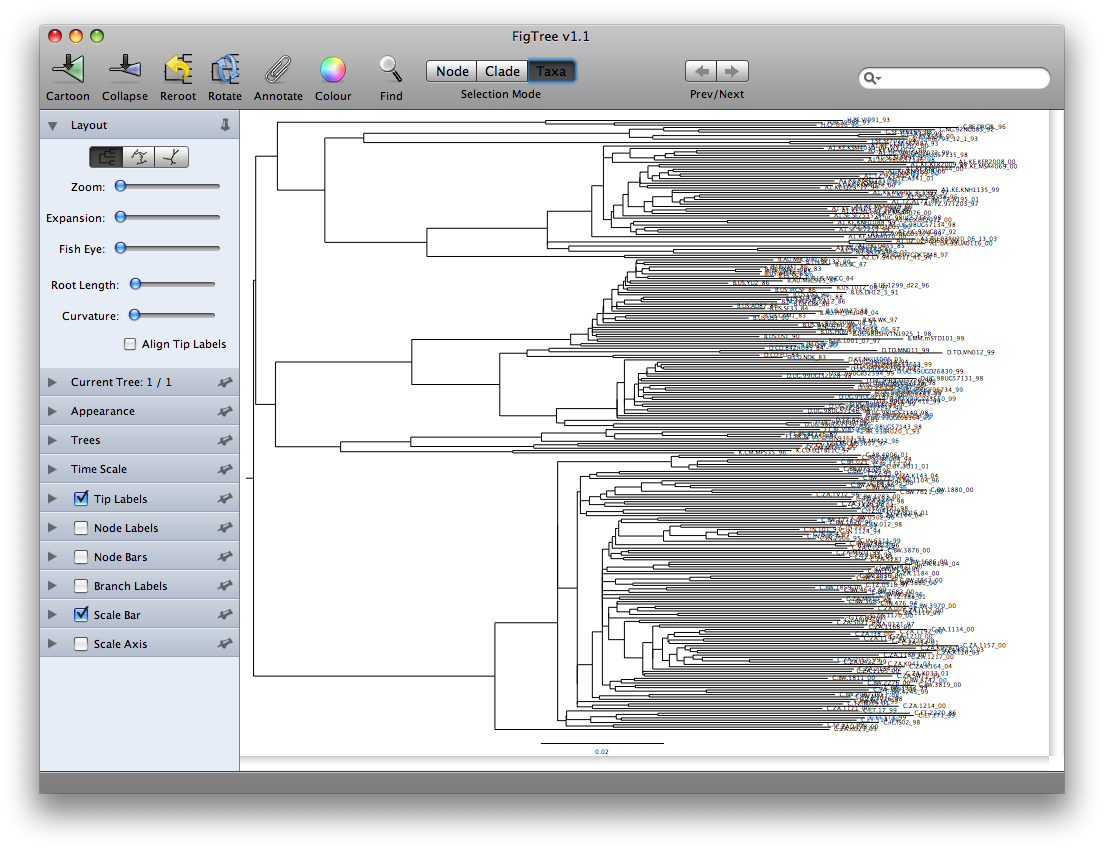
\includegraphics[scale=.2]{figtree.png}
\end{center}
\end{frame}

\section{FreePhyloTree}

\begin{frame}{Propósito}
\begin{itemize}
\item Software a mi medida.
\item Herramienta científica y educativa.
\item Editable por los usuarios, a lo wiki.
\item Dato geográficos, bibliografía, cladogramas y/o filogenias
  alternativas, etcétera.
\item Principal problema, la BD $\rightarrow$ yo solo no puedo hacerlo.
\end{itemize}
\end{frame}

\begin{frame}{Estrategia}
\begin{block}{Estado actual}
Herramienta que construye cladogramas desde wikispecies. El «aprendizaje» reside
en wikipedia. El árbol organiza la información.

Problema $\rightarrow$ no es adecuado para el propósito final de la aplicación.
\end{block}

\begin{block}{Futuro}
\begin{enumerate}
\item Atraer usuarios.
\item Cambiar la plataforma y «volcar» lo aprovechable de wikispecies.
\item Los usuarios conquistados «me ayuden».
\end{enumerate}

Problema $\rightarrow$ ni idea de programación web. Más ayudantes.
\end{block}
\end{frame}

\begin{frame}{Evolución}
\begin{itemize}
\item Aprender openGL, libcurl, Qt, algoritmos de visualización
  de grafos, cmake, protocolo http, $\ldots$.
\item De Ogre a openGL, de openGL con SDL a openGL con Qt. Rama
  3D. Experimentación con c++0x.
\item De fichas de taxones en wikipedia a exploración de wikispecies.
\item Cada artículo de wikispecies es «de su padre y de su madre».
\item Por lo general, buena aceptación de la aplicación.
\end{itemize}
\end{frame}

\begin{frame}{Fin}
\begin{center}
\Huge{Preguntas}\\
\vspace*{2ex}
\tiny{http://freephylotree.blogspot.com/}\\
\tiny{http://gitorious.org/freephylotree}\\
\tiny{http://cusl5-freephylo.forja.rediris.es/}\\
\vspace*{5ex}
\Huge{Gracias}
\end{center}
\end{frame}

\end{document}
